\documentclass{report}

% Chargement des packages utilisés.
% Packages pour la langue et le caractères.
\usepackage[utf8]{inputenc}
\usepackage[T1]{fontenc}
\usepackage[francais]{babel}
\usepackage{lmodern}

% Images.
\usepackage{graphicx}

% Packages pour les formules mathématiques.
\usepackage{amsmath}
\usepackage{amssymb}
\usepackage{mathrsfs}

% Fin du chargement des packages.

% Meta-data du document.
\title{3D OpenGL : Résumé du cour 1}
\author{Clément \bsc{Barbaste}}
\date{24 janvier 2014}
% Fin Meta-data.

\begin{document}
\maketitle
\part{Rappel géometrie}
\chapter{Vecteurs}
\section{Rappel des opérations de base sur les vecteurs}
\subsection{Définition d'un vecteur}
Un vecteur défini une direction dans l'espace. Un vecteur est défini par 3 coordonnées. Soit le vecteur $\vec{U} = \{U_x, U_y, U_z\}$ définie par 3 coordonnées, avec les points $A = \{A_x, A_y, A_z\}$ et $B = \{B_x, B_y, B_z\}$ à ses extrémitées :
\[
\vec{U} = 
\left|
\begin{array}{rcl}
  U_x &=& B_x - A_x\\
  U_y &=& B_y - A_y\\
  U_z &=& B_z - A_z
\end{array}
\right|
\]
\subsection{Addition et Multiplication d'un scalaire}
Soit le vecteur $\vec{U}$.
\[
\begin{array}{rcl}
\vec{U}\times1.5 &=& 
\left|
\begin{array}{c}
	U_x\times1.5\\
	U_y\times1.5\\
	U_z\times1.5
\end{array}
\right|\\\\
\vec{U} + \vec{V} &=&
\left|
\begin{array}{c}
	U_x+V_x\\
	U_y+V_y\\
	U_z+V_z
\end{array}
\right|
\end{array}
\]
\subsection{Norme d'un vecteur}
Soit le vecteur $\vec{U}$ avec à ses extrémitées les point A et B tel que $\vec{U} = \vec{AB}$.
La norme de $\vec{U}$ noté $\|\vec{U}\|$ vaut :
\[
  \|\vec{U}\| = \sqrt{U_{x}^{2} + U_{y}^{2} + U_{z}^{2}}
\]
$\|\vec{U}\|$ = distance entre A et B.\\
Si $\|\vec{U}\|$ = 1, alors $\vec{U}$ est \textbf{normé}.\\
Pour obtenir un vecteur $\overrightarrow{Un}$, normé et de même direction que $\vec{U}$ :
\[
\overrightarrow{Un} = 
\left |
\begin{array}{rcl}
    Un_x &=& \frac{U_x}{\|\vec{U}\|}\\
    Un_y &=& \frac{U_y}{\|\vec{U}\|}\\
    Un_z &=& \frac{U_z}{\|\vec{U}\|}
\end{array}
\right |
\]
\subsection{Produit scalaire}
Le produit scalaire entre 2 vecteurs $\vec{U}$ et $\vec{V}$ se note : $\vec{U}\cdot\vec{V}$
\[
\begin{array}{rcl}
\vec{U} \cdot \vec{V} &=& U_{x} \times V_{x} + U_{y} \times V_{y} + U_{z} \times V_{z}\\
\text{ou} \\
\vec{U} \cdot \vec{V} &=& \cos \alpha \times \|\vec{U}\| \times \|\vec{V}\|
\end{array}
\]

\subsection{Produit vectoriel}
Le produit vectoriel entre 2 vecteurs $\vec{U}$ et $\vec{V}$ se note : $\vec{U} \wedge \vec{V}$
\[
\vec{U} \wedge \vec{V} =
\left|
\begin{array}{rcl}
  U_y \times V_{z} &-& U_{z} \times V_y\\
  U_z \times V_{x} &-& U_{x} \times V_z\\
  U_x \times V_{y} &-& U_{y} \times V_x
\end{array}
\right|
\]
Relation entre le produit vectoriel et l'angle:
\[
\|\vec{U} \wedge \vec{V}\| = \sin \alpha \times \|\vec{U}\| \times \|\vec{V}\|
\]

\subsection{Propriétés importantes}
\begin{tabular}{rcl}
Symétrie &$\to$& $\vec{U} \cdot \vec{V} = \vec{V} \cdot \vec{U}$\\
Distributivité &$\to$& $\vec{U} \cdot (\vec{V}+\vec{W}) = \vec{U} \cdot \vec{V} + \vec{U} \cdot \vec{W}$\\
Homogénéité &$\to$& $(\lambda \vec{U}) \cdot \vec{V} = \lambda(\vec{U} \cdot \vec{V})$\\
lien avec la norme &$\to$& $\vec{U} \cdot \vec{U} = \|\vec{U}\|^2$\\
Orthogonalité &$\Longleftrightarrow$& $\vec{U} \cdot \vec{V} = 0$ $\Leftrightarrow$ $\alpha = 90$\degre ou 270\degre\\
Colinéarité &$\Longleftrightarrow$& $\|\vec{U} \wedge \vec{V}\| = 0$ $\Leftrightarrow$ $\alpha = 0$\degre ou 180\degre\\
\end{tabular}

\chapter{Matrices}
\section{Rappel des opérations de base sur les matrices}
\subsection{Définition d'une matrice}
Soit A une matrice $m \times n$, $m$ étant le nombre de \textbf{lignes} et $n$ le nombre de \textbf{colonnes} :
\[
 A = 
 \begin{pmatrix}
  a_{1,1} & a_{1,2} & a_{1,3} & \dots & a_{1,n}\\
  a_{2,1} & a_{2,2} & a_{2,3} & \dots & a_{2,n}\\
  a_{3,1} & a_{3,2} & a_{3,3} & \dots & a_{3,n}\\
  \vdots & \vdots & \vdots & \vdots & \vdots\\
  a_{m,1} & a_{m,2} & a_m{m,3} & \dots & a_{m,n}
 \end{pmatrix}
\]

Une matrice peut être vue comme un vecteur vertical, avec les coordonnées du vecteur.
ex:
\[
 \vec{U} = 
 \begin{pmatrix}
  U_x\\
  U_y\\
  U_z
 \end{pmatrix}
\]

\subsection{Addition et multiplication entre matrices}
Soit les matrices A et B.
\begin{tabular}{cc}
 $A = \begin{pmatrix} a_{1,1} & a_{1,2} \\ a_{2,1} & a_{2,2} \end{pmatrix}$ & $B = \begin{pmatrix} b_{1,1} & b_{1,2} \\ b_{2,1} & b_{2,2} \end{pmatrix}$
\end{tabular}\\
\begin{math}
 A + B = \begin{pmatrix}
          a_{1,1} + b_{1,1} & a_{1,2} + b_{1,2}\\
          a_{2,1} + b_{2,1} & a_{2,2} + b_{2,2}
         \end{pmatrix}
\end{math}\\
\begin{math}
 A \times B = \begin{pmatrix}
          a_{1,1} \times b_{1,1} +  a_{1,2} \times b_{2,1} & a_{1,1} \times b_{1,2} +  a_{1,2} \times b_{2,2}\\
          a_{2,1} \times b_{1,1} +  a_{2,2} \times b_{2,1} & a_{2,1} \times b_{1,2} +  a_{2,2} \times b_{2,2}
         \end{pmatrix}
\end{math}
\subsection{Multiplication d'une matrice et d'un scalaire}
\begin{math}
 \lambda \times A = \begin{pmatrix}
          \lambda \times a_{1,1} & \lambda \times a_{1,2}\\
          \lambda \times a_{2,1} & \lambda \times a_{2,2}
         \end{pmatrix}
\end{math}


%%%%%%%%%%%%%%%%%%%%%%%%%
%	Partie 2	%
%%%%%%%%%%%%%%%%%%%%%%%%%
\part{Géometrie 2D-3D}
\chapter{Projections}
  Il existe plusieurs types de projection, ellse seront rappellés dans les section à suivre.
\section{Projection orthogonale}
\subsection{Projection d'un point sur une droite}
Soit une droite $d$ définie par 2 points $A$ et $B$. Ainsi que $C$, le point à projeter sur la droite $d$. Le point projeté se nomme $C'$.
Par Pytagore, on sait que:
\[ \frac{\|\overrightarrow{AC'}\|}{\|\overrightarrow{AC}\|} = \cos \alpha\]\\
D'après la \emph{section 1.1.4}:
\[\frac{\overrightarrow{AC}\cdot \overrightarrow{AB}}{\|\overrightarrow{AC}\| \times \|\overrightarrow{AB}\|} = \cos \alpha\]
On peut en deduire:
\[ 
\|\overrightarrow{AC'}\| = \frac{\overrightarrow{AC} \cdot \overrightarrow{AB}}{\|\overrightarrow{AB}\|}
\]
Maintenant qu'on a la norme de $\overrightarrow{AC'}$, il nous faut projeter le point $C$ sur $d$. Pour cela il suffit de translater $A$ par $\overrightarrow{AB}$ normé, avec une distance $\|\overrightarrow{AC'}\|$.
On notera ce vecteur normé $\vec{u}$, pour vecteur \emph{U}nitaire.
\[
\begin{array}{rcl}
 C'_x &=&  A_x + Ux \times \|\overrightarrow{AC'}\|\\
 C'_y &=&  A_y + Uy \times \|\overrightarrow{AC'}\|\\
 C'_z &=&  A_z + Uz \times \|\overrightarrow{AC'}\|
\end{array}
\]
\subsection{Projection d'un point sur un plan}
Soit le plan $P$ défini par le point $A$ et le vecteur normal $\vec{n}$. Ainsi que le point $B$, à projeter sur le plan. Le point projeté se nomera $B'$.
\[
\frac{\|\overrightarrow{BB'}\|}{\|\overrightarrow{BA}\|} = \cos \alpha
\]
D'après la \emph{section 1.1.4}:
\[
 \frac{\overrightarrow{BA} \cdot \overrightarrow{n}}{\|\overrightarrow{BA}\| \times \|\overrightarrow{n}\|} = \cos \alpha
\]
On en deduit:
\[
 \|\overrightarrow{BB'}\| = \frac{\overrightarrow{BA} \cdot \overrightarrow{n}}{\|\overrightarrow{n}\|}
\]
Maintenant qu'on a la norme de $\overrightarrow{BB'}$, il suffit de translater $B$ par $\vec{n}$ normé (qu'on nommera $\vec{u}$), avec une distance $\|\overrightarrow{BB'}\|$.
\[
 \begin{array}{rcl}
  B'_x &=& B_x - n_x \times \|\overrightarrow{BB'}\|\\
  B'_y &=& B_y - n_y \times \|\overrightarrow{BB'}\|\\
  B'_z &=& B_z - n_z \times \|\overrightarrow{BB'}\|
 \end{array}
\]
\chapter{Transformation}
\section{Translation}
On applique une translation avec un vecteur $\vec{U}$ à chaque point de l'objet, les liaisons entre les points restent les mêmes.
\section{Mise à l'échelle}
On choisit un point $C$ dans l'espace, puis on fait une multiplication scalaire, par un ratio $r$, sur chaque vecteurs avec, $C$, et un sommet de la figure à mettre à l'échelle, aux extrémitées.
Si le point $C$ n'est pas au centre de la figure, celle-ci sera déformée par la mise à l'echelle.
\section{Rotations}
En supposant un point $A = \{A_x, A_y, A_z\}$, et que l'angle de rotation se nomme $\alpha$.
\subsection{Rotation par l'axe OX}
On considère le point comme une matrice \{3,1\}
\[
 A = 
 \begin{pmatrix}
  A_x\\
  A_y\\
  A_z
 \end{pmatrix}
\]
Puis pour appliquer la rotation, multiplie la matrice $A$ par la matrice de rotation en $\overrightarrow{Ox}$.
\[
\begin{array}{rcl}
 A' &=& rotOx \times A\\
 A' &=& 
 \begin{pmatrix}%matrice rotOX
  1 & 0 & 0\\
  0 & \cos \alpha & - \sin \alpha\\
  0 & \sin \alpha & \cos \alpha
 \end{pmatrix}
 \begin{pmatrix}
  A_x\\
  A_y\\
  A_z
 \end{pmatrix}
  =
  \begin{pmatrix}
   A'_x\\
   A'_y\\
   A'_z
  \end{pmatrix}
 \end{array}
\]
\subsection{Rotation par l'axe OY}
Identique que pour OX, sauf pour la matrice de rotation qui est:
\[
 \begin{pmatrix}
  \cos \alpha & 0 & \sin \alpha\\
  0 & 1 & 0\\
  -\sin \alpha & 0 & \cos \alpha
 \end{pmatrix}
\]
\subsection{Rotation par l'axe OZ}
Identique que pour OX, sauf pour la matrice de rotation qui est:
\[
 \begin{pmatrix}
  \cos \alpha & -\sin \alpha & 0\\
  \sin \alpha & \cos \alpha & 0\\
  0 & 0 & 1
 \end{pmatrix}
\]
\subsection{Rotation autour d'un axe quelconque}
On suppose que l'axe de rotation est le vecteur unitaire $\vec{u}$.
Voici la matrice de rotation:
\[
 \begin{pmatrix}
  u_x^2 + (1 - u_x^2) \cos \alpha & u_x u_y (1 - \cos \alpha) - u_z \sin \alpha & u_x u_z (1 - \cos \alpha) + u_y \sin \alpha\\
  u_x u_y (1 - \cos \alpha) + u_z \sin \alpha & u_y^2 + (1 - u_y^2) \cos \alpha & u_y u_z (1 - \cos \alpha) - u_x \sin \alpha\\
  u_x u_z (1 - \cos \alpha) - u_y \sin \alpha & u_y u_z (1 - \cos \alpha) + u_x \sin \alpha &  u_z^2 + (1 - u_z^2) \cos \alpha
 \end{pmatrix}
\]

\part{Notions de cour}
\chapter{Notions sur les objets 3D}
\section{Etapes de conception}
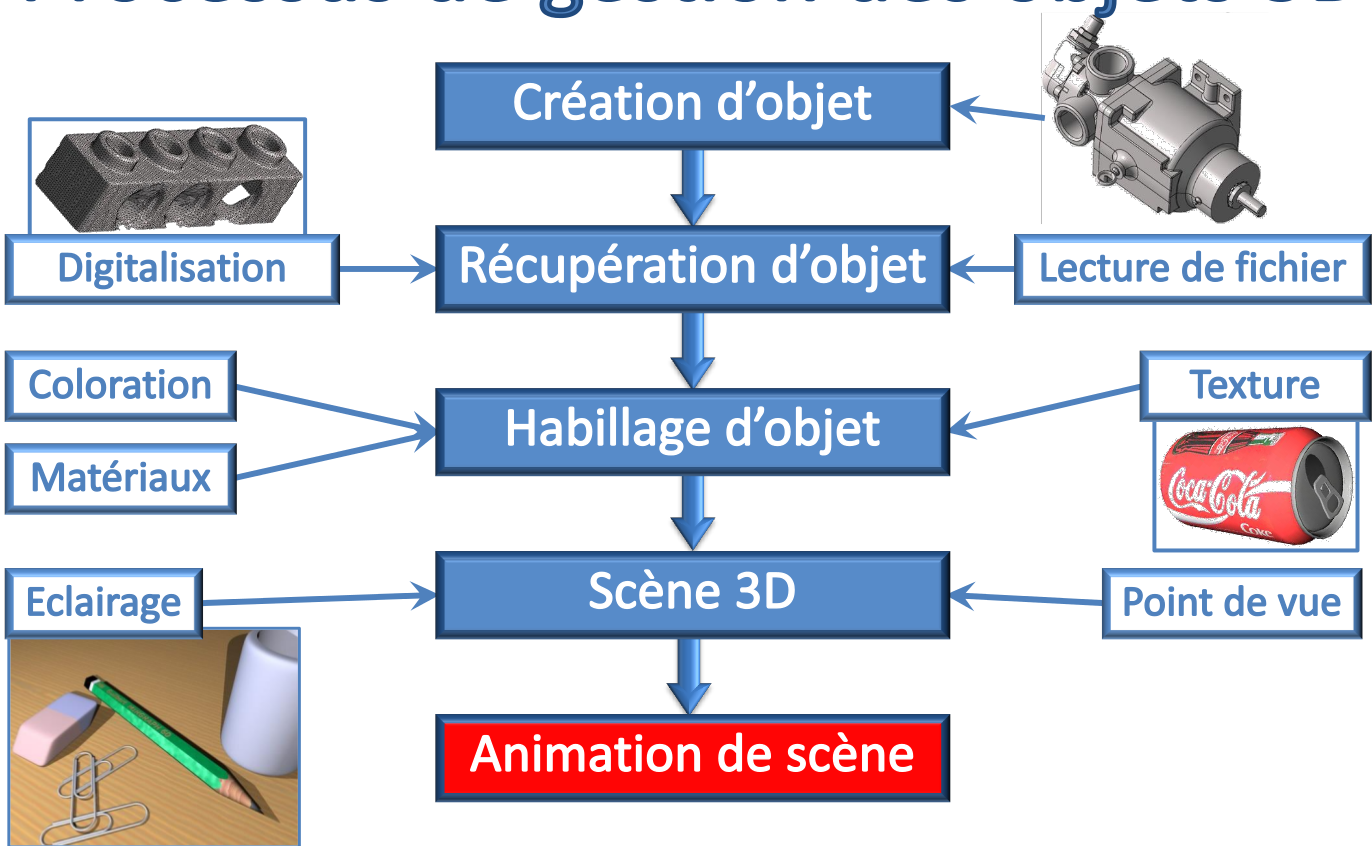
\includegraphics[width=400px]{./schema_conception.png}
\section{Différentes formes de 3D}
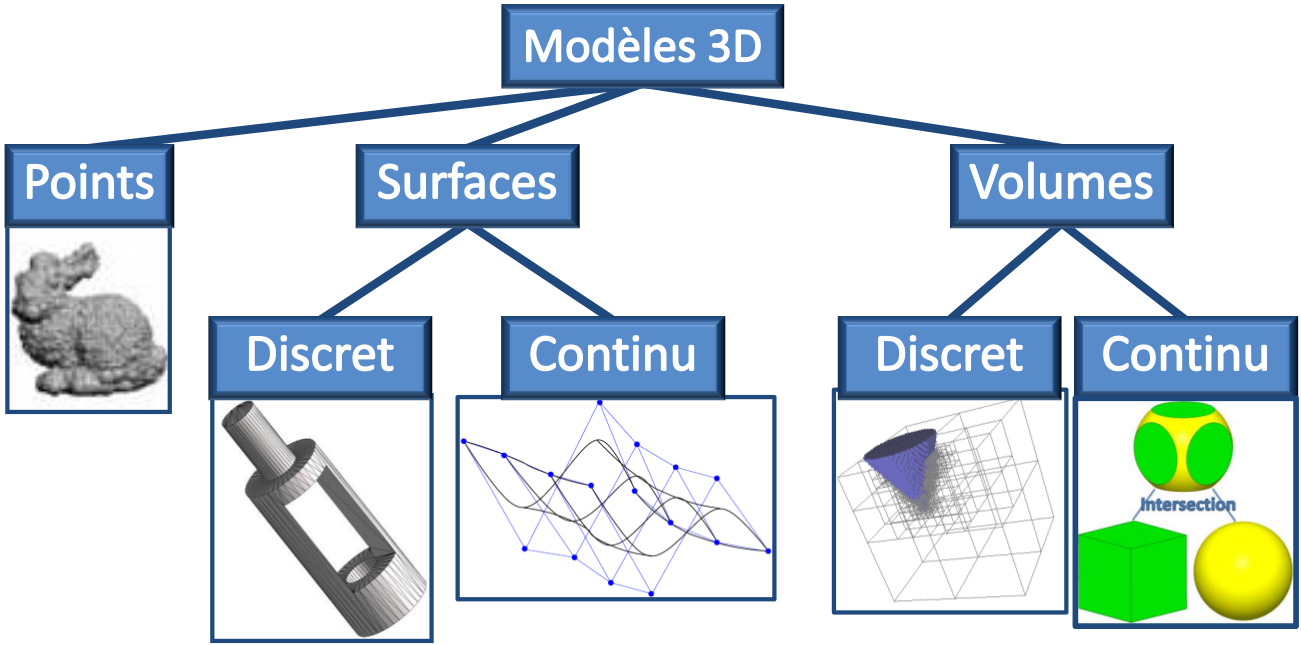
\includegraphics[width=400px]{./dif_3d.png}
\section{Fonctions importantes de glub}

\end{document}